
	\subsection{Аргумент Майера-Виеториса}

	\begin{definition} 
		Пусть $M$~--- многообразие размерности $n$. Его открытое покрытие $\{ U_{\alpha} \}_{\alpha}$ называется \emph{хорошим}, если все конечные пересечения $U_{\alpha_0} \cap \ldots U_{\alpha_n}$ диффеоморфны $\R^n$. 
	\end{definition}

	\begin{theorem} 
		Любое многообразие имеет хорошее покрытие. 
	\end{theorem}
	\begin{proof}[Набросок доказательства]
		Во-первых, для этого нам понадобится риманова метрика на многообразии. То, что любое гладкое многообразие метризуемо, следует например из теоремы вложения Уитни. Или, например, можно взять покрытие $M$ координатными шарами $U_{\alpha}$, взять гладкую риманову метрику (пулбек стандартного скалярного произведения) $\langle  \cdot, \cdot \rangle_{\alpha}$ из них и сложить с весами из разбиения единицы, подчиненного покрытию $U_{\alpha}$: 
		\[
			\langle \cdot, \cdot \rangle = \sum_{\alpha} \rho_{\alpha} \langle \cdot, \cdot \rangle_{\alpha}. 
		\]

		Так вот, как только у нас есть разбиение единицы, известно, что каждая точка в многообразии имеет геодезически выпуклую окрестность. Тогда, если мы возьмём покрытие геодезически выпуклыми окрестностями (каждая из них диффеоморфна $\R^n$), все конечные пересечения будут диффеоморфны $\R^n$, как мы и хотели. 
	\end{proof}

	\begin{statement} 
			Если многообразие $M$ имеет конечное хорошее покрытие, тогда его когомологии де Рама (и компактные когомологии) конечномерны. 
	\end{statement}	
	\begin{proof}
		Будем использовать индукцию по покрытию и последовательность Майера-Виеториса. 

		\noindent\bf{Шаг 1.} Запишем последовательность Майера-Виеториса:

		\begin{center}
			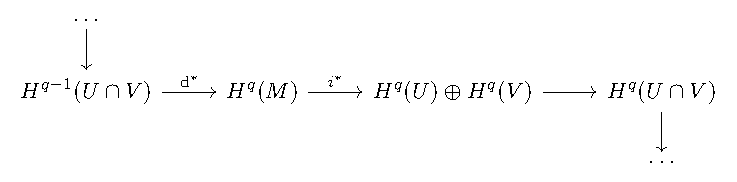
\includegraphics{lectures/7/pictures/cd_17.pdf}
		\end{center}		

		Заметим, что $H^q(M) \cong \Im{i^*} \oplus \Ker{i^*} \cong \Im{i^*} \oplus \Im{\mathrm{d}^*}$ по точности последовательности. Тогда ясно, что если когомологии $U, V$ и  $U \cap V$ конечномерны, то  $H^q(M)$ тоже конечномерны. 

		\noindent\bf{Шаг 2.} Теперь запустим индукцию по мощности покрытия. Пусть утверждение верно для любого многообразия, допускающего хорошее покрытие из не более чем $k$ элементов. Рассмотрим многообразие $M$, имеющее хорошее покрытие из $(k + 1)$-го элемента $\{ U_0, \ldots, U_k \}$. 

		Положим $U = U_p, \ V = U_0 \cup U_1 \cup \ldots \cup U_{p - 1}$. Тогда по индукционному предположению $H^q(U), \ H^q(V), \ H^q(U \cap V)$ конечномерны, откуда по шагу 1 $H^q(U \cup V)$ конечномерны, что мы и хотели.  
 	\end{proof}	

 	\subsection{Двойственность Пуанкаре}

 	Пусть $V$ и $W$ конечномерные векторные пространства. Напомним, что спаривание 
 	\[
 		\langle \cdot, \cdot \rangle\colon  V \otimes W \to \R 
 	\]
 	 называется \emph{невырожденным}, если 
 	 \[ 
 	 	\langle v, w \rangle = 0 \ \forall w \in W \implies v = 0.
 	 \]
 	 Заметим, что это эквивалентно тому, что отображение $v \mapsto \langle v, \cdot \rangle$ определяет изоморфизм $V \cong W^*$.


 	 \begin{theorem}[Двойственность Пуанкаре] 
 	 	Пусть $M$~--- ориентируемое многообразие размерности $n$. Тогда 
 	 	\[
 	 		\forall q \quad H^q(M) \cong \lr*{ H^{n - q}_{c}(M) }^*.
 	 	\]
 	 \end{theorem}
 	 \begin{remark}
 	 	Мы докажем это в случае, когда $M$ обладает конечным хоршим покрытием, но вообще, это ограничение не по существу (так как принцип Майера-Виеториса можно обобщить на произвольные ориентируемые многообразия). То есть, сформулироавнное в теореме верно и без условия на конечномерность когомологий (но, доказывать это мы не будем). 
 	 \end{remark}
 	 \begin{proof}
 	 	Для ориентируемого многообразия мы можем определить спаривание 
 	 	\[
 	 		\int\limits_{M}\colon H^q(M) \otimes H_{c}^{n - q}(M) \to \R, \ [\omega] \otimes [\alpha] \mapsto \int\limits_{M} \omega \wedge \alpha  
 	 	\]

 	 	Тут мы по существу пользуемся ориентируемостью, так как интегрирование корректно продолжается на когомологии при помощи теоремы Стокса. 

 	 	Мы будем доказывать, что определённое выше спаривание невырождено. Для этого нам понадобится несколько лемм. 

 	 	Напомним сначала 5-лемму: 

 	 	\begin{lemma}[5-лемма] 
 	 		Рассмотрим диаграмму 
 	 		\begin{center}
 	 			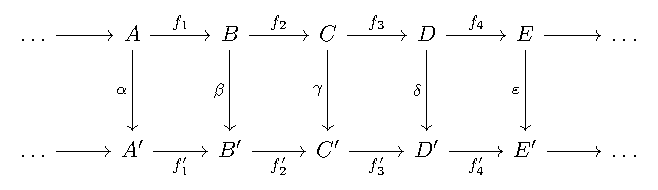
\includegraphics{lectures/7/pictures/cd_18.pdf}
 	 		\end{center}

 	 		Предположим, что строки точны и $\alpha, \beta, \delta, \varepsilon$~--- изоморфизмы. Тогда $\gamma$ тоже изоморфизм. 
 	 	\end{lemma}

 	 	\begin{lemma} 
 	 		Следующая диаграмма коммутативна с точностью до знака: 

 			\begin{center}
 				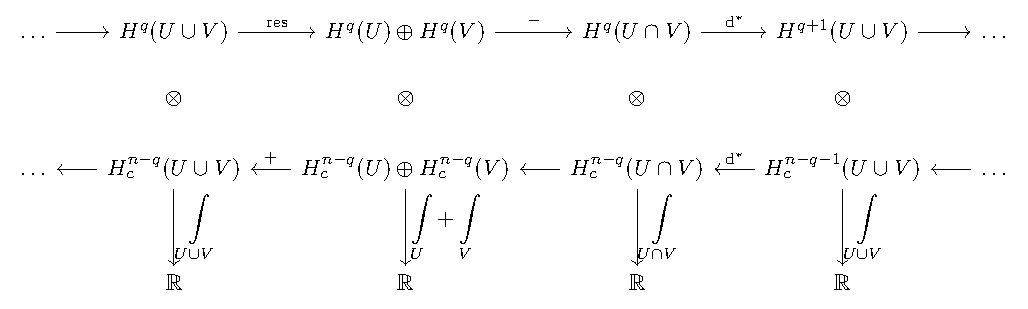
\includegraphics{lectures/7/pictures/cd_19.pdf}
 			\end{center}
 	 	\end{lemma}
 	 	\begin{proof}[Доказательство леммы]

 	 	коммутативность с точностью до знака тут означает следующее: например, если мы возьмём $\omega \in H^q(U \cap V)$ и $\tau \in H^{n - q - 1}_{c}(U \cup V)$, то 
 	 	\[
 	 		\int\limits_{U \cap V} \omega \wedge \mathrm{d}_* \tau = \pm \int\limits_{U \cup V} \mathrm{d}^* \omega \wedge \tau.
 	 	\]
 	 	Это означает, что взять форму из верхнего этажа третьего столбца  и пойти направо, а потом вниз -- это то же самое, что взять форму из нижнего этажа четвертого столбца и пойти направо, а потом вверх. 

 	 	Проверим например, коммутативность правого квадрата (для левых квадратов тут немного проще). Возьмём $\omega H^{q}(U \cap V)$, $\tau \in H^{n - q - 1}(U \cup V)$. Напомним, что мы знаем явный вид кограничного связывающего гомоморфизма:

 	 	\[
 	 		 \mathrm{d}^*\omega = \begin{cases} -\mathrm{d}(\rho_V \omega), & \text{ на } U \\ \mathrm{d}(\rho_U \omega), & \text{ на } V \end{cases}, \quad \mathrm{d}_* \tau = \begin{cases} \mathrm{d}(\rho_U \tau ), & \text{ на } U \\ \mathrm{d}(\rho_U \omega), & \text{ на } V \end{cases}. 
 		 \]	 

 		 Заметим, что так как эти формы из когомологий, они замкнутые, а тогда 
 		 \[
 		 	\mathrm{d}(\rho_V \omega) = \mathrm{d}\rho_V \wedge \omega + \rho_v \mathrm{d}\omega = \mathrm{d}\rho_V \wedge \omega.  
 		 \]
 		 \[
 		 	\mathrm{d}(\rho_V \tau) = \mathrm{d}\rho_V \wedge \tau + \rho_V \mathrm{d}\tau = \mathrm{d}\rho_V \wedge \tau.
 		 \]
 		 Тогда то, что нам нужно показать сводится к перестановке сомножителей во внешнем произведении 
 		 \[
 		 	\int\limits_{U \cap V} \omega \wedge \mathrm{d}_* \tau = \int\limits_{U \cap V} \omega \wedge \mathrm{d}\rho_V \wedge \tau = (-1)^{\deg{\omega}} \int\limits_{U \cap V} \mathrm{d}\rho_V \wedge \omega \wedge \tau = (-1)^{\deg{\omega} + 1} \int\limits_{U \cap V} \mathrm{d}^* \omega \wedge \tau.
 		 \]

 		 С другой стороны, так как $\supp\lr*{\mathrm{d}^* \omega } \subseteq U \cap V$. 

 		  Теперь заметим, что приведённая выше лемма означает, что диаграмма ниже коммутативна с точностью до знака: 

 		  \end{proof}

 	 \begin{center}
 	 	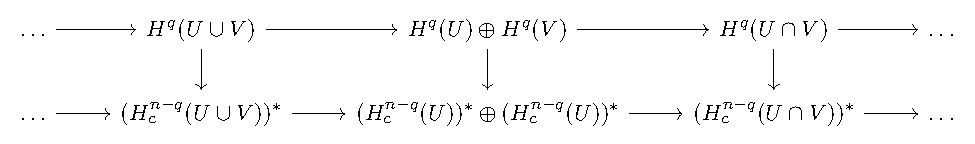
\includegraphics{lectures/7/pictures/cd_20.pdf}
 	 \end{center}

 	Если пристально посмотреть на эту диаграмму, можно заметить, что из 5-леммы следует, что если мы знаем, что двойственность Пуанкаре выполнена для $U, V, U \cap V$, то мы знаем это и для $U \cup V$. 

 	Теперь осталось запустить индукцию по размеру хорошего покрытия: 

 	\noindent\bf{База.} Если $M \cong \R^n$, то двойственность Пуанкаре следует из лемм Пуанкаре: 
 	\[
 		H^q(\R^n) = \begin{cases} \R, & q = 0 \\ 0, & \text{ иначе } \end{cases}, \quad \quad H^{q}_{c}(\R^n) = \begin{cases} \R, & q = n \\  0, & \text{ иначе } \end{cases}.
 	\]

 	\noindent\bf{Переход.} Делается также, как в теореме про конечномерность когомологий. 
 	 \end{proof}

 	 \begin{remark}
 	 	Обратное утверждение, то есть, что 
 	 	\[
 	 		H^{q}_c(M) \cong \lr*{H^{n - q}(M)}^*,
 	 	\]
 	 	верно не всегда. Это связано с тем, что 
 	 	\[
 	 		M = \bigsqcup_{i = 1}^{\infty} M_i \implies H^q(M) = \prod_{i = 1}^{\infty} H^q(M_i), \quad H^q_c(M) \cong \bigoplus_{i = 1}^{\infty} H^q(M_i) .
 	 	\]
 	 	Но, для компактных многообразий утверждений сохранится. 
 	 \end{remark}

 	 Из двойственности Пуанкаре сразу следует такой замечательный результат: 
 	 \begin{theorem} 
 	 	Пусть $M$~--- связное ориентированное многообразие размерности $n$. Тогда $H^n_c(M) = \R$. В частности,  если $M$ компактно, то $H^n(M) = \R$.
 	 \end{theorem}
 	 \begin{proof}
 	 	В самом деле, по двойственности Пуанкаре $H^n_c(M) \cong (H^{n - n}(M))^* \cong \R^* \cong \R$. 
 	 \end{proof}



 	 \subsection{Формула Кюннета}

 	 Из двойственности Пуанкаре также можно не слишком сложным образом получить формулу Кюннета: 

 	 \begin{theorem}[Формула Кюннета] 
 	 	Пусть $M$ и $N$~--- многообразия. Тогда имеет место следующий изоморфизм градуированных колец: 
 	 	\[
 	 		H^{\bullet}(M \times N) \cong H^{\bullet}(M) \otimes H^{\bullet}(N).
 	 	\]
 	 	или же, иными словами, 
 	 	\[
 	 		H^{n}(M \times N) \cong \bigoplus_{p + q = n} H^p(M) \otimes H^q(N).
 	 	\]
 	 \end{theorem}
 	 \begin{proof}
 	 	Будем опять пользоваться принципом Майера-Виеториса и 5-леммой. Пусть $U$ и $V$~--- открытые подмножества в $M$, запишем точную последовательность Майера-Виеториса: 
 	 	\begin{center}
 	 		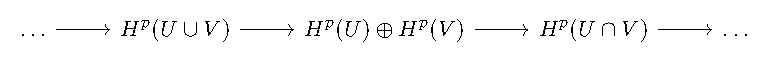
\includegraphics{lectures/7/pictures/cd_21.pdf}
 	 	\end{center}

 	 	Тензорно умножим её на $H^{n - p}(N)$ (так как тензорное произведение -- это точный функтор, последовательность останется точной), получим диаграмму 

 	 	\begin{center}
 	 		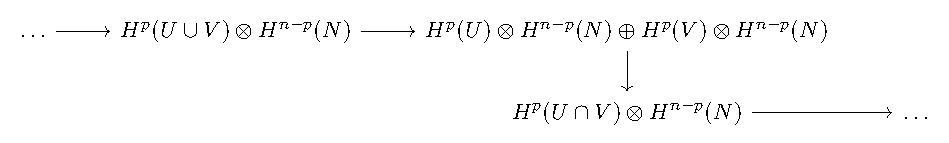
\includegraphics{lectures/7/pictures/cd_22.pdf}
 	 	\end{center}

 	 	Просуммируем по $p$ от $0$ до $n$, получим точную последовательность 
 	 	\begin{center}
 	 		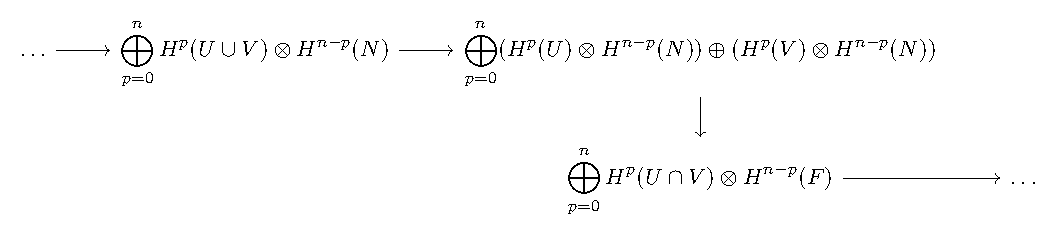
\includegraphics{lectures/7/pictures/cd_23.pdf}
 	 	\end{center}

 	 	Теперь заметим, что у нас есть следующая коммутативная диаграмма: 

 	 	\begin{center}
 	 		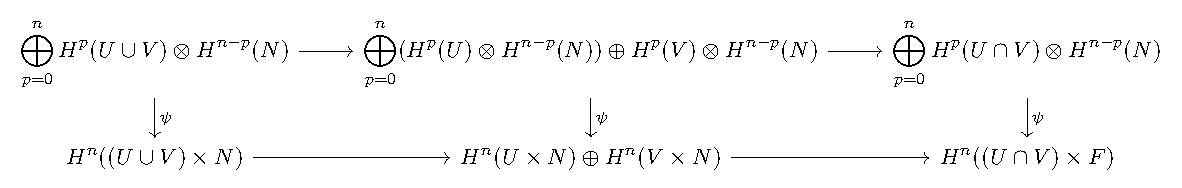
\includegraphics[scale = 0.95]{lectures/7/pictures/cd_24.pdf}
 	 	\end{center}
 	 	где $\psi$ определён так: у нас есть проекции на обе координаты ,
 	 	\begin{center}
 	 		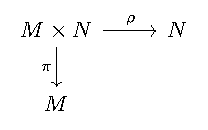
\includegraphics{lectures/7/pictures/cd_25.pdf}
 	 	\end{center}
 	 	они естественным образом индуцируют отображение 
 	 	\[
 	 		\omega \otimes \varphi \mapsto \pi^*\omega \wedge \rho^*\varphi.
 	 	\]
 	 	Это отображение и индуцирует нужное нам отображение в когомологиях: 
 	 	\[
 	 		\psi\colon H^{\bullet}(M) \otimes H^{\bullet}(N) \to H^{\bullet}(M \times N).
 	 	\]

 	 	Так вот, в диаграмме выше нужно проверить какую-то коммутативность. Вообще говоря, нужно проверить коммутативность квадратов, например вот этого 

 	 	\begin{center}
 	 		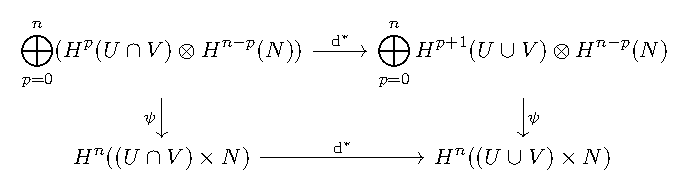
\includegraphics{lectures/7/pictures/cd_26.pdf}
 	 	\end{center}

 	 	Но, делать это очень уж лень. Это делается стандартным образом, короче. 

 	 	Так вот, по 5-лемме мы опять получаем, что если формула Кюннета верна для $U, V, U \cap V$, то она верна и для $U \cap V$. Далее нужно заметить, что в случае $\R^n$ утверждение следует из леммы Пуанкаре, а дальше нужно сделать такой же индукционный переход, как и в теореме ранее. 

 	 \end{proof}

 	 Похожими техниками можно получить следующее важное обобщение: 

 	 \begin{theorem}[Лере, Хирш] 
 	 		Пусть $E$~--- локально тривиальное расслоение над $M$ со слоем $F$. Предположим, что нашлись классы $e_1, \ldots, e_n \in H^{\bullet}(E)$ такие, что для любого вложения слоя $i\colon F \hookrightarrow E$ их пулбеки $i^*(e_1), \ldots, i^*(e_n)$~--- базис $H^{\bullet}(F)$ как векторного пространства над $\R$, то $\{ e_1, \ldots, e_n \}$~--- базис $H^{\bullet}(E)$, как векторного пространства над $H^{\bullet}(M)$ и 
 	 		\[
 	 			H^{\bullet}(M) \otimes H^{\bullet}(F) \cong H^{\bullet}(E).
 	 		\]
 	 \end{theorem}

 	 

 	